% !TEX root = ../thesis.tex

\chapter{Methodology}
	\label{chap:typesetting}
	In order to apply any ML and NLP to the tweet dataset, to see if we could do any information extraction and statistical analysis, we first needed to be able to generate a ranking of the ten tweets we had obtained. We sourced the tweets themed around Brexit on Twitter, and then a pipeline (see fig: \ref{fig:pipeline}) for sourcing peoples preferences of the tweets was created. The pipeline created was handled by the web app. The web app allowed the user to create an account and then compare the tweets. The resulting decision updated the ELO rating for each tweet and the more simplified traditional comparison judgment method. Each user gets only presented five different combinations, ensuring that a single tweet was only seen by the user once.
	
	\begin{figure}[b]
		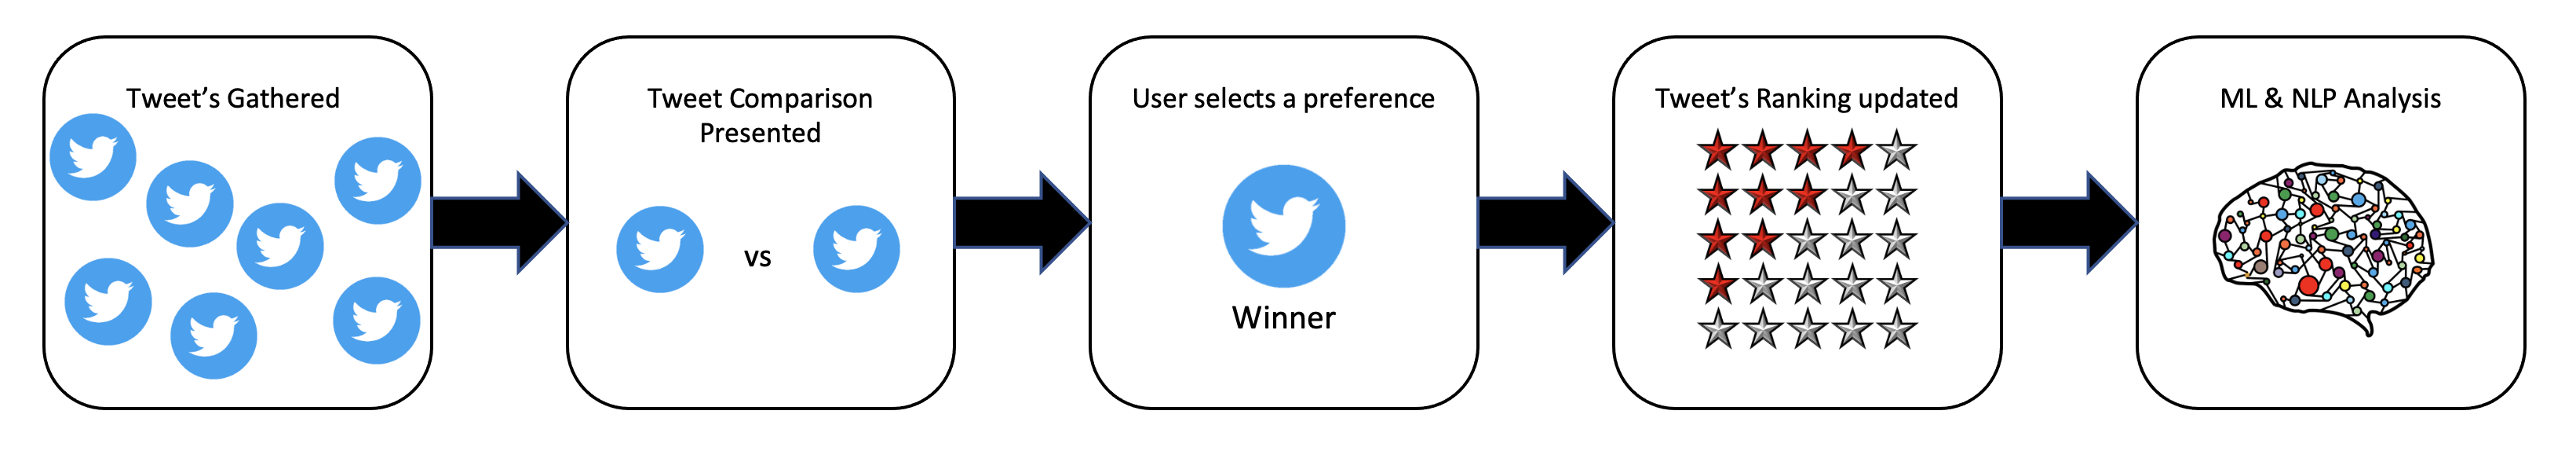
\includegraphics[width=\textwidth]{pipline.png}
		\caption{A visual representation of the processes pipline.}
		\label{fig:pipeline}
		
	\end{figure}

	\section{Overview of Application}
	
	\subsection{Web Application}
	The application has two main sections. The first section is a web application. This web application aims to rank the ten Twitter tweets by presenting users with two tweets and asking them which one is better. In essence, the web application is a tool to crowdsource data on peoples views based on the tweets that they get presented. The web app then creates two ranking systems. One ranking system uses an ELO system, and one the users a more pairwise comparative judgement style. The pairwise comparative judgement score gets calculated by the total wins getting subtracted by the total losses. 
	
	The second section is an exploratory Python notebook looking into NLP tasks on the tweets. We carry out sentiment analysis and information extraction on the tweets to see if any patterns within the tweets match their ranking's place. For example, positive sentiment tweets getting a higher ranking with a particular theme, other than Brexit possibly showing. The ultimate aim is to create a tweet marking rubric based on the results and the information. Additionally, we will then aim to see if we can use the gained knowledge from the information extraction to see if we can train ML models to predict the tweets position within the marking grid accurately.
	
	\subsection{NLP Information Extraction}
	
	\subsubsection{Part of Speach Tagging}
	
	
	\subsubsection{Named Entity Recognition}
	
	
	\subsubsection{Feature Extraction}
	Feature extraction aims to transform tokens into features. An excellent technique to achieve this is a bag of words (BOW). This technique will count the occurrences of a particle token within our text. Therefore, for each token, we will have a feature column. This feature column gets referred to as text vectorisation. However, using a standard BOW will lose the word order, and the counters can not be normalised. 
	
	In order to preserve some order, we can count the tokens as pairs or triplets, for example. This technique gets also referred to as n-grams. The n refers to the number of tokens to get referenced. Some examples are 1-grams for tokens and 2-grams for token pairs. However, this has its problems as it can create too many features. A solution to this problem is to remove some n-grams from the feature set. This solution can get achieved by using the metric based on the frequency of their occurrence.
	
	The n-grams that we would want to remove based on their frequency are high and low-frequency n-grams. High-frequency grams get usually referred to as stop words, and low-frequency grams are rare words or typos. We especially want to remove the low-frequency n-grams as they can create overfitting. Ultimately, we ideally want the medium frequency words.
	
	A technique we can use to find the medium frequency n-grams is term frequency-Inverse document frequency (TF-IDF). TF-IDF has two main stages, the term frequency (TF) and the inverse document frequency (IDF). The TF ($tf(t,d)$) looks for the frequency of the n-gram (term) $t$ in the document $d$ \cite{sarkar2016text}. While IDF takes the total number of documents in the corpus ($N = |D|$) and the number of documents where the term t appears ($|\{d \varepsilon D:t \varepsilon d\}|$) \cite{sarkar2016text}. So the IDF gets represented as $idf(t,D) = \log\frac{N}{|\{d \varepsilon D:t \varepsilon d\}|}$ \cite{sarkar2016text}. TF-IDF ($tdidf(t,d,D) = tf(t,d) \cdot idf(t,D)$) achieves a high weight by a high-term frequency, within a given document, and a low  document frequency of the term in the whole collection of documents \cite{sarkar2016text}.
	
	Through using TF-IDF, we can replace counters within our BOW with the TF-IDF value. We can then normalise the result row-wise by dividing by $L_2-norm$. Through this method, important features will have a relatively high value. Through this method, we are then able to display the key features within our documents.
	
	
	\subsubsection{Sentiment Analysis}
	
	\subsection{Text Similarity} %Scoring
	Text similarity scoring aims to analyse and measure how close two entities of text are to each other \cite{sarkar2016text}. We can compare two objects. By comparing these objects, it is then possible to predict how similar they are. We can use docs, spans, tokens or Lexeme to calculate the similarity score \cite{spacy_vec_sim}. To measure the similarity scores between text entities, we can use two main types of methods, term and document similarity \cite{sarkar2016text}. 
	
	Predicting similarity helps build recommendation systems or flag duplicates. For example, it allows for the system to suggest user content that's similar to what they are currently looking at or label a support ticket as a duplicate if it is very similar to an already existing one \cite{spacy_vec_sim}. Additionally, similarity measures are an excellent way to take the noisy text data and group the text together. It allows us to see what text gets considered similar to each other by using unsupervised clustering techniques \cite{sarkar2016text}.
	
	As the dataset we are dealing with are Twitter tweets, we decided to do this through entire document similarity and spans of named entities to see if the results provide us with any insights in terms of providing any feedback to the user. 
	
	
	\subsubsection{Utterence Pattern Matching}
	
	\subsubsection{Finding Word Sequence Patterns}
	
	\subsubsection{Key Phrases}
	The Key phrases method aims to take a document object and find the word or phrase with the most information to it. This technique is effective, especially when creating a chatbot. Key phrases allow the computer to determine what the user, who is interacting with the chatbot, is talking about. A single word in the question can sometimes be enough, but we might need to look at phrases. Key phrases work well with dependency parsing \cite{vasiliev2020natural}.
	
	We decided to experiment with this feature to see if we could extract the key phrases from the tweets and see if they could provide us with any insights and present them to the user as feedback.
	
	\section{Tools}
	To create the web application and insights from the tweets, we required to use several tools. It is a requirement that we develop a full-stack web application with a user UI, an area to input the user's judgements on the tweet, store the results using a database, and extract information from the tweets using NLP techniques. Several factors within the final application needed to be satisfied for the tools to be appropriate for use.
	
	%needs adapting - taken from CSCM10 Spec %%%%%%
	We will be using Trello for the kanban tools. "Kanban" is the Japanese word for "visual signal" \cite{kanbanmeaning}. Using Kanban boards allows us to keep our work visible, this is to allow others to see what it is we are doing, and what is needed to get done. These will allow everyone to see the full picture and keep everyone on the same page.
	
	David Anderson discovered that kanban boards get split into five components: Visual signals, columns, work-in-progress limits, a commitment point, and a delivery point \cite{anderson2010kanban}.
	
	Kanban teams write all their project's work items onto cards, and these are usually one per card. The kanban board gets split into columns, with each column representing an activity which composes the workflow. All the cards change between the workflow until the activity is complete. The column workflow titles can be as simple as to do, in progress and completed. However, David suggests that there should be a work in progress (WIP) limit \cite{anderson2010kanban}. When a column has reached the limit, of three cards, all team members get expected to focus on the cards in progress. The WIP limits are critical for exposing bottlenecks in the workflow and maximizing flow. WIP limits give an early warning sign that too much work is commissioned. Backlogs of ideas are where the ideas of the team and the customers get placed. The moment an idea gets picked up by a team member and work begins, this gets referred to as the commitment point \cite{anderson2010kanban}. When the product is finished and ready for deployment, this stage is referred to as the delivery point. The overall aim of the kanban is to take a card from the commitment point to delivery point as quick as possible. 
	%%%%%%%%%%%%%%%
	
	
	\subsection{Programming Language}
	While many programming languages can handle creating a full-stack application and conducting ML, for example, Java \cite{arnold2005java}, Php \cite{bakken2000php} and JavaScript \cite{flanagan2006javascript}. We decided to use the Python language \cite{Python}. We decided upon Python due to our familiarity with it over the other main languages and its versatility. We made this decision because Python can make full-stack applications with the use of additional libraries and handle most NLP ML tasks using libraries like NLTK \cite{loper2002nltk}, SpaCy \cite{spacy2}, Sci-Kit Learn \cite{scikit-learn}, and TensorFlow \cite{tensorflow2015-whitepaper}.
	
	\subsection{Libraries}
	While we use the Python programming language to create the web application and the NLP information extraction, we require significantly different libraries to complete each task. We will look into the potential web libraries available to us and the NLP focused libraries. We will then present the libraries that we decided upon for each of the parts.
	
	\subsubsection{Web Application}
	For creating the web application, there were two main libraries available. These were Django and Flask.
	
	Django is a high-level Python Web framework that encourages rapid development and clean, pragmatic design. Built by experienced developers, it takes care of much of the hassle of Web development, so you can focus on writing your app without needing to reinvent the wheel. It’s free and open source \cite{django}.
	
	While Flask is a small framework by most standards—small enough to be called a “micro- framework,” and small enough that once you become familiar with it, you will likely be able to read and understand all of its source code \cite{grinberg2018flask}. 
	
	Flask has three main dependencies. The routing, debugging, and Web Server Gateway Interface (WSGI) subsystems come from Werkzeug; the template support is provided by Jinja2; and the command-line integration comes from Click. These dependencies are all authored by Armin Ronacher, the author of Flask \cite{grinberg2018flask}. 
	
	Flask has no native support for accessing databases, validating web forms, authenti‐ cating users, or other high-level tasks. These and many other key services most web applications need are available through extensions that integrate with the core pack‐ ages. As a developer, you have the power to cherry-pick the extensions that work best for your project, or even write your own if you feel inclined to. This is in contrast with a larger framework, where most choices have been made for you and are hard or sometimes impossible to change \cite{grinberg2018flask}.
	
	%decision and justification
	After experimenting with the two frameworks, we decided upon Flask. Flask got decided upon because of the short time frame to put the project together. Additionally, the lightweight nature of the framework also played a fact. As this will be just an initial prototype, Django's other requirements would be unessential additionals to the project. Therefore, taking focus away from what we believe is the main focus. 
	
	\subsubsection{NLP Tasks}
	There are several NLP library packages already available within Python, all having pros and cons. The most popular and influential libraries are Natural Language Toolkit (NLTK), Gensim, CoreNLP, spaCy, TextBlob, Pattern and PyNLPi.
	
	% NLTK
	NLTK is one of the leading platforms for building Python programs that can work with human language data. It presents a practical introduction to programming for language processing. NLTK comes with a host of text processing libraries for sentence detection, tokenisation, lemmatisation, stemming, parsing, chunking, and POS tagging.NLTK is one of the leading platforms for building Python programs that can work with human language data. It presents a practical introduction to programming for language processing. NLTK comes with a host of text processing libraries for sentence detection, tokenisation, lemmatisation, stemming, parsing, chunking, and POS tagging.
	
	NLTK provides easy-to-use interfaces to over 50 corpora and lexical resources. The tool has the essential functionalities required for almost all kinds of natural language processing tasks with Python.
	
	%Gensim
	Gensim is a Python library designed specifically for “topic modeling, document indexing, and similarity retrieval with large corpora.” All algorithms in Gensim are memory-independent, w.r.t., the corpus size, and hence, it can process input larger than RAM. With intuitive interfaces, Gensim allows for efficient multicore implementations of popular algorithms, including online Latent Semantic Analysis (LSA/LSI/SVD), Latent Dirichlet Allocation (LDA), Random Projections (RP), Hierarchical Dirichlet Process (HDP) or word2vec deep learning. 
	
	Gensim features extensive documentation and Jupyter Notebook tutorials. It largely depends on NumPy and SciPy for scientific computing. Thus, you must install these two Python packages before installing 
	Gensim.
	
	% CoreNLP
	Stanford CoreNLP comprises of an assortment of human language technology tools. It aims to make the application of linguistic analysis tools to a piece of text easy and efficient. With CoreNLP, you can extract all kinds of text properties (like named-entity recognition, part-of-speech tagging, etc.) in only a few lines of code. 
	
	Since CoreNLP is written in Java, it demands that Java be installed on your device. However, it does offer programming interfaces for many popular programming languages, including Python. The tool incorporates numerous Stanford’s NLP tools like the parser, sentiment analysis, bootstrapped pattern learning, part-of-speech (POS) tagger, named entity recogniser (NER), and coreference resolution system, to name a few. Furthermore, CoreNLP supports four languages apart from English – Arabic, Chinese, German, French, and Spanish.
	
	%spaCy
	spaCy is an open-source NLP library in Python. It is designed explicitly for production usage – it lets you develop applications that process and understand huge volumes of text. 
	
	spaCy can preprocess text for Deep Learning. It can be be used to build natural language understanding systems or information extraction systems. spaCy is equipped with pre-trained statistical models and word vectors. It can support tokenisation for over 49 languages. spaCy boasts of state-of-the-art speed, parsing, named entity recognition, convolutional neural network models for tagging, and deep learning integration.
	
	% TextBlob
	TextBlob is a Python (2 \& 3) library designed for processing textual data. It focuses on providing access to common text-processing operations through familiar interfaces. TextBlob objects can be treated as Python strings that are trained in Natural Language Processing.
	
	TextBlob offers a neat API for performing common NLP tasks like part-of-speech tagging, noun phrase extraction, sentiment analysis, classification, language translation, word inflection, parsing, n-grams, and WordNet integration.
	
	%Pattern
	Pattern is a text processing, web mining, natural language processing, machine learning, and network analysis tool for Python. It comes with a host of tools for data mining (Google, Twitter, Wikipedia API, a web crawler, and an HTML DOM parser), NLP (part-of-speech taggers, n-gram search, sentiment analysis, WordNet), ML (vector space model, clustering, SVM), and network analysis by graph centrality and visualisation. 
	
	Pattern can be a powerful tool both for a scientific and a non-scientific audience. It has a simple and straightforward syntax – the function names and parameters are chosen in a way so that the commands are self-explanatory. While Pattern is a highly valuable learning environment for students, it serves as a rapid development framework for web developers.
	
	% PyNLPi
	Pronounced as ‘pineapple,’ PyNLPl is a Python library for Natural Language Processing. It contains a collection of custom-made Python modules for Natural Language Processing tasks. One of the most notable features of PyNLPl is that it features an extensive library for working with FoLiA XML (Format for Linguistic Annotation).
	
	PyNLPl is segregated into different modules and packages, each useful for both standard and advanced NLP tasks. While you can use PyNLPl for basic NLP tasks like extraction of n-grams and frequency lists, and to build a simple language model, it also has more complex data types and algorithms for advanced NLP tasks. 
	
	%Conclusion/Final decision
	%All taken from: https://www.upgrad.com/blog/python-nlp-libraries-and-applications/
	Although NLTK, TextBlob was used in some experimenting, we decided to use spaCy as the main NLP library. However, NLTK was used on the side (especially with their stop words). As one of the key things we wanted to do was to extract information from the tweets, spaCy allowed us to do this and prepare the data for deep learning. While we did not need a very deep Recurrent Neural Network (RNN), we did implement one to complete the sentiment analysis on the tweets. We used an RNN with two things in mind, to see how well it could perform on small amounts of text, like a tweet, and with the future thoughts of it being able to handle large amounts of text, like someone's essay in an exam.
	
	
	
	
	\subsection{IDE}
	While many great IDEs are available like Pycharm, Jupyter Lab, Atom and Sublime, we decided to use VS Code. The decision behind this was that it allowed us to explore code within interactive python notebooks (ipynb) and standard python scripts. Additionally, it allowed us to create HTML, CSS, and Javascript files within the same IDE.
	
	
	\section{Ranking System}
	
	As discussed in the literature review, along with a more traditional pairwise comparative judgment algorithm, we could choose either an ELO or Glicko system. While each has advantages and disadvantages, we decided to use the ELO system. We decided to use this system as we felt it would be more robust for how we intend to be calculating the tweet scores, as we will be taking random pairings of tweets that will only be seen once by the user. Only seeing the tweet appear once removes any opportunity for a user to underrate a tweet because it has been seen multiple times without losing its impact. 
	
	Due to this reason, the ELO system, with its probability aspect to the scoring, helped determine outcomes on potential unseen tweet combos. While not considering if a tweet gets seen more than any others, this would have a massive impact on the comparative judgement pairwise comparison method.
	
	
	\begin{figure}[t]
		\centering
		 Prob A Wins$ = 1/1+10^{(B-A/400)}$
		\caption{To calculate the expected score for a tweet.}
		\label{fig:elo_maths_1}
	\end{figure}

\begin{figure}[t]
	\centering

	new score $= rating + 32 * $  score $ - $ expected score
	\caption{A visual representation of the web apps navigation.}
	\label{fig:elo_maths_2}
\end{figure}
	
	\section{Data Set}
	There were two datasets used within this study. The primary dataset was the ten tweets gathered from Twitter, with a theme of being a joke based on Brexit. The other dataset was the IMDB sentiment analysis dataset. This dataset got used to train and test our RNN model before using our tweets on it. 
	
	\subsection{Data Capture Method}
	Twitter's developer API got used to allow for the tweets to get extracted. Additionally, the library [name here] got also used. The tweets were then uploaded to the Firebase database through a Python Notebook for the main web app to access them. Having the tweets in the database also allowed us to be then able to create a notebook to then access the data to then do the NLP investigating within.
	
	\subsection{Pre-Processing}
	
	
	
	
	\section{Implementation}
	%[gather tweets]
	
	%[Web App]
	The web application got implemented using the Python web library Flask. The web application used several industry-standard tools, for example, HTML, CSS, JavaScript, Bootstrap and dynamic content. The HTML, CSS, Bootstrap and JavaScipt was used to handle the application's front end. The web application had a mesh style navigation system (see fig: \ref{fig:web_app_nav}). However, when the user was on the compare page, this would push to itself and update the users content based on what they had next in their comparison list.
	
	\begin{figure}[t]
		\centering
		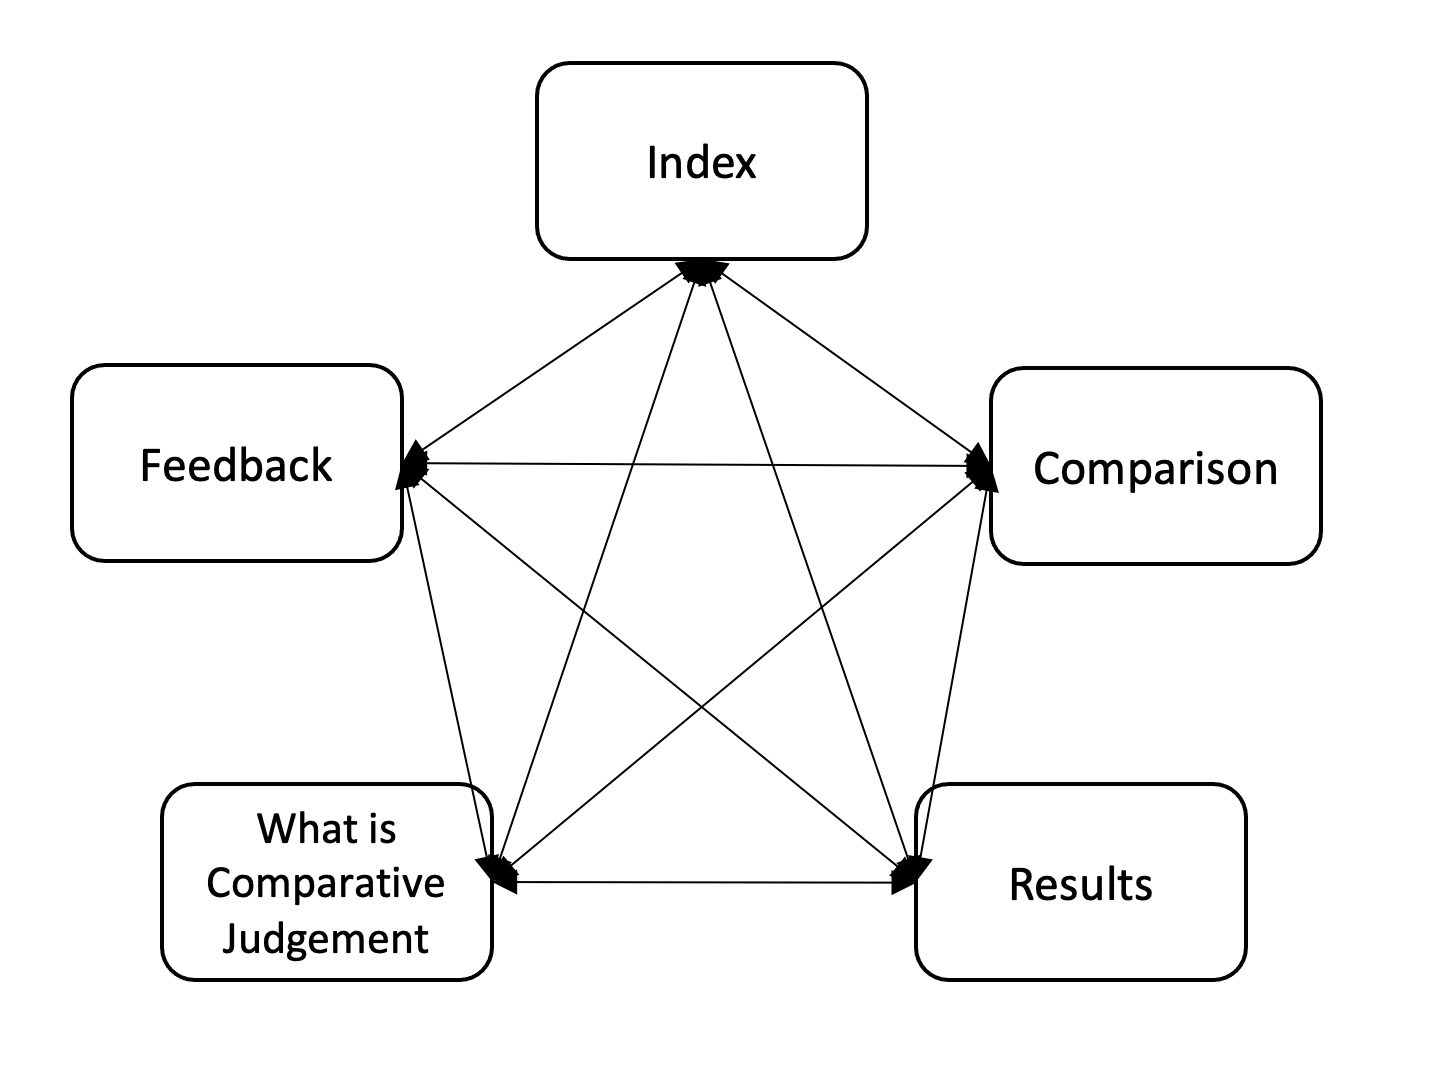
\includegraphics[width=8cm]{web_app_nav.png}
		\caption{A visual representation of the web apps navigation.}
		\label{fig:web_app_nav}
		
	\end{figure}
	
	Additional tools like Google's Firebase was used to handle user authentication and store the web app's content in their real-time databases. The real-time databases are a NoSQL document notation database that updates in real-time. 
	
	A requirement of the app is for the user to be able to create an account. The account sign-up only requires an email and will generate all the additional requirements for the other parts of the app to work in the background. They are linking all the results for these comparisons to the user's ID. At the point of sign-up, a user position within the comparison cycle gets generated, a random selection of tweets to get compared against will be generated. The logic behind the sampling is that a user will only see a single tweet once. Therefore making sure that the user sees these tweets for the first time, every time, making it more of a fair comparison.
	
	Heroku handled the hosting of the web app. Heroku is a free-to-use web hosting provider. However, with it being a free-to-use service, it did bring about some undesirable aspects, mainly the website's slow loading time.
	
	%[Tweet Comparison Presentation]
	As previously mentioned, a user will have a random sample of the tweets, which will have a unique pairing. Therefore ensuring that a user will only see one tweet within the pairing once, to make the tweet's joke not lose its impact as the second or third time a user sees the same tweet, it naturally would lose its edge. Hence, each user will have their own predetermined set of comparisons at the point of sign-up but will one see, for example, tweet one once. As we mentioned, this was to keep the tweets fresh for the user and make them more likely to complete all the comparisons. Otherwise, if the user had to see all unique comparisons, they would have to see 45 different combinations in total just for ten different tweets. So if we put this into the context of a teacher, who would usually have 30 students in a class, several teachers will have to see 435 different combinations, which is just for one class. When this gets factored in, we are looking at around 11175 for 150 different students.
	
	The app will query the database and look for the user's current position when presenting the tweets. Based on their position, the tweet combinations then get checked for that according to the round. The tweet ids are then queried against the tweets' content and then presented to the web page. The user gets expected to select a tweet that they find funnier and then provide an opportunity to justify their choice, which is optional.   
	
	When the user presses the "Vote!" button, this saves the results to the database, updating the two result systems and the user's position. The process will save which tweet won and lost and update the ELO ranking and the standard ranking. The standard ranking gets calculated by taking how many times a tweet has won minus the number it has lost. The implementation of the standard ranking system is to try to implement a more traditional comparative judgement ranking system. In contrast, the ELO system is using a more traditional approach (see fig: \ref{fig:elo_maths}) Which gets updated after every comparison. The implementation of the two systems allows us to see if the ELO or more standard version of CJ is the more effective one or if they naturally mirror each other.
	
	\begin{figure}[t]
		\centering
		$ Prob A Wins = 1/1+10^{(B-A/400)}$
		\caption{To calculate the expected score for a tweet.}
		new score $= rating + 32 * $  score $ - $expected score
		\caption{A visual representation of the web apps navigation.}
		\label{fig:elo_maths}
		
	\end{figure}
	
	This process gets repeated until the user has completed all five comparisons.
	
	\section{Designs}
	
	\subsection{Home Page}
	
	\subsection{Comparison Page}
	
	\subsection{What is Comparative Judgement Page}
	
	\subsection{Results Page}
	
	\subsection{Feedback Page}
	
	
	\section{Risks}
	
	\begin{center}
		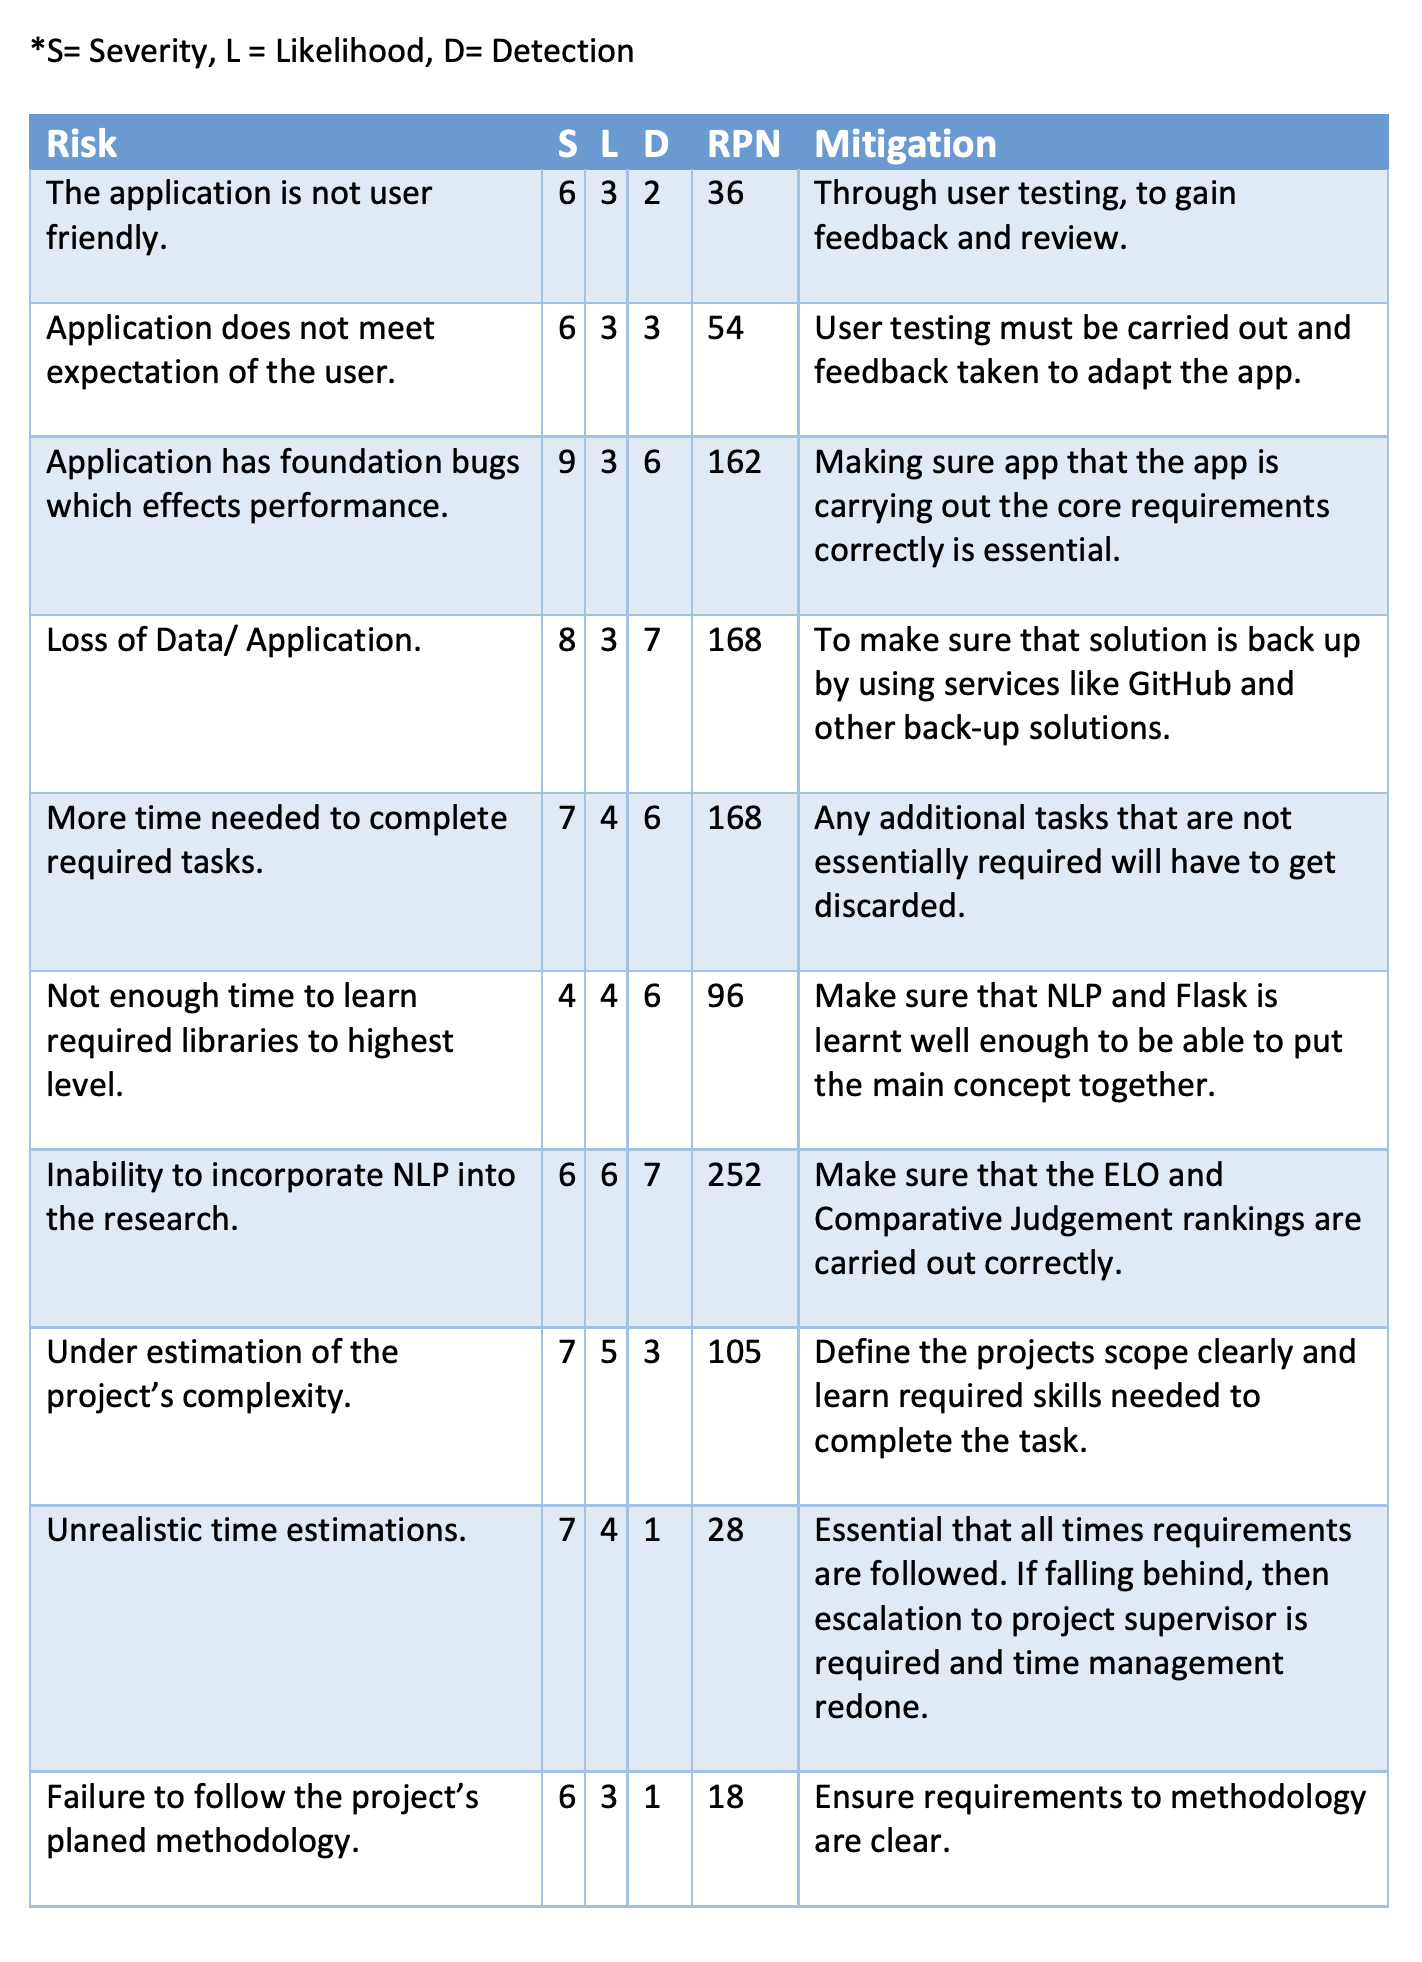
\includegraphics[width=13cm]{risk_table.png}
		%\caption{A visual representation of the processes pipline.}...
	\end{center}
		
	
	
	
	\begin{landscape}
		\section{Schedule}
		\begin{center}
			\item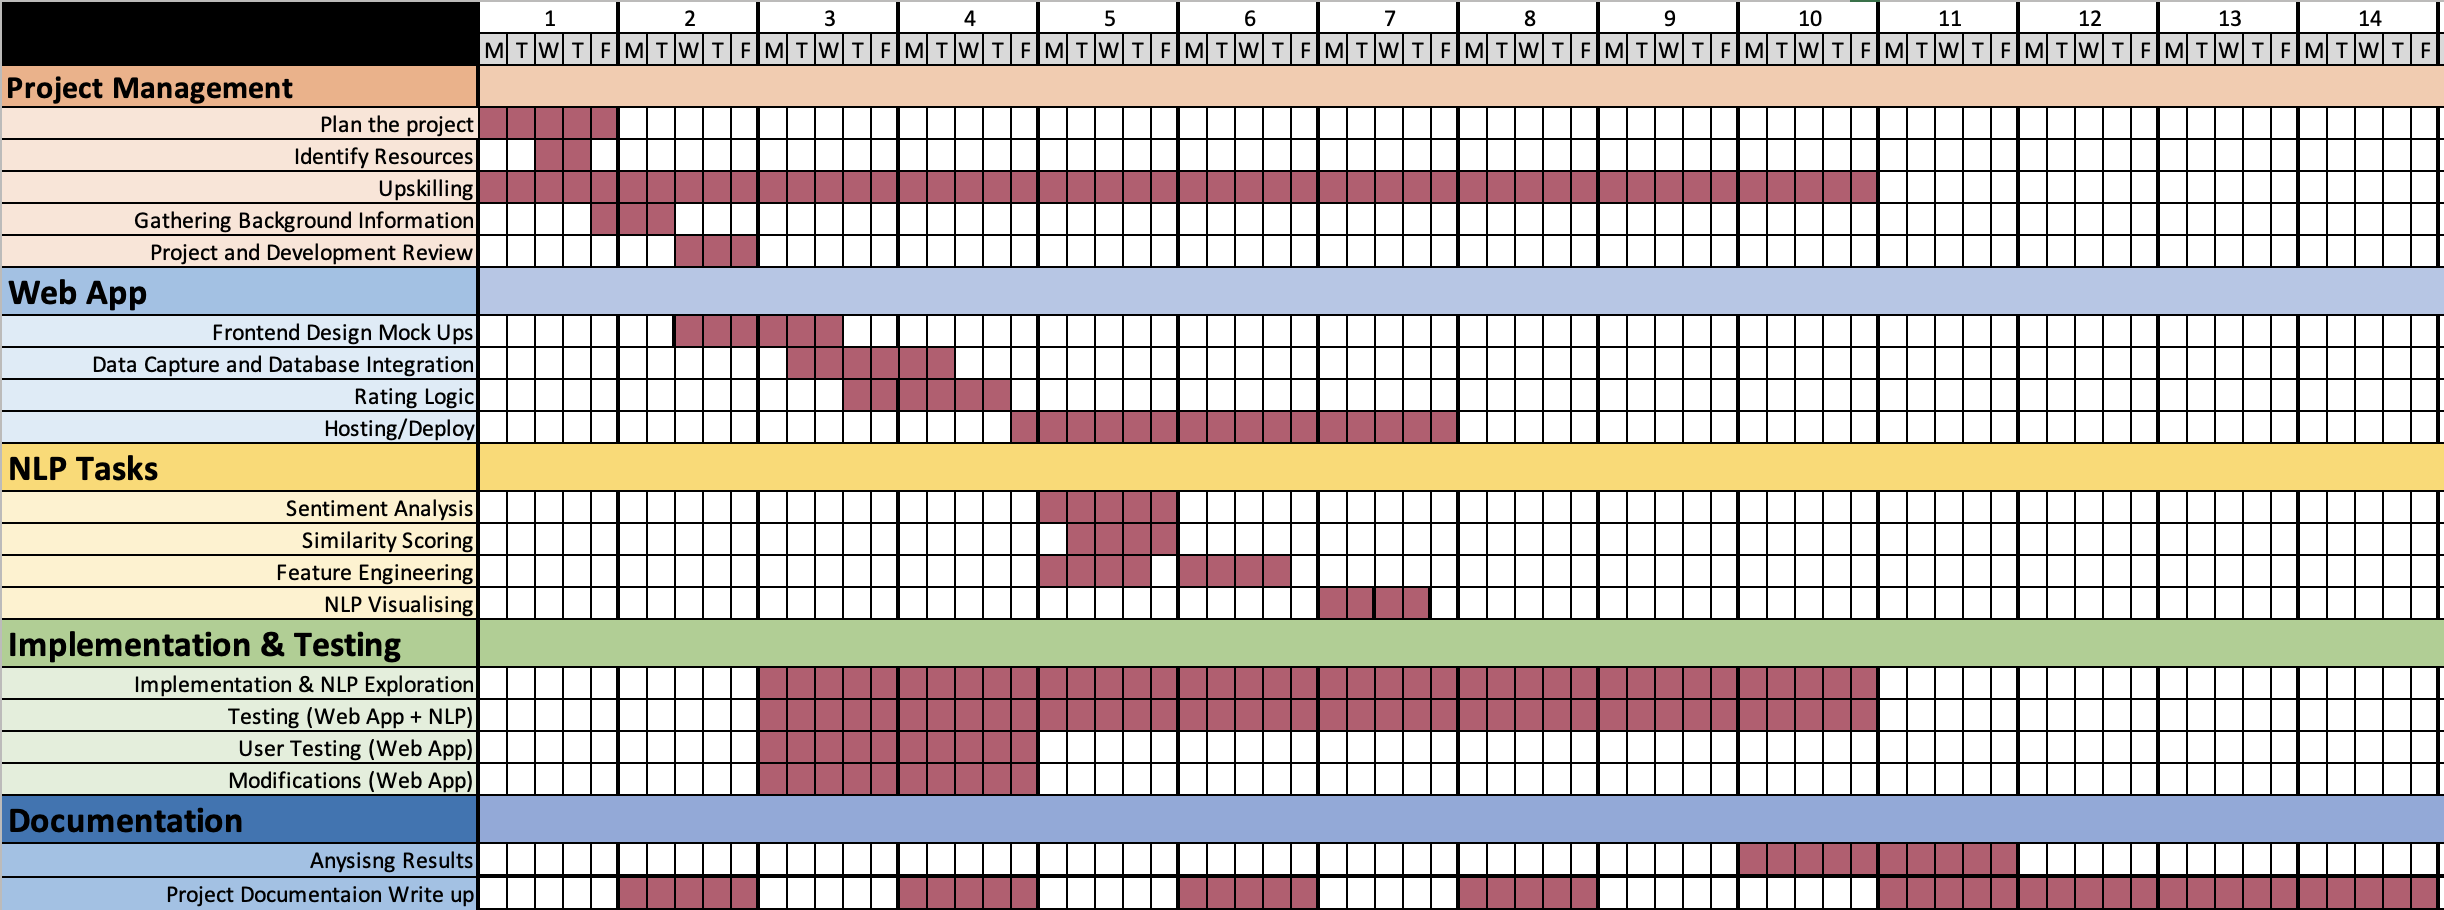
\includegraphics[width=21cm]{ganttchart.png}
		\end{center}
	\end{landscape}
	
	\section{Software Development Life Cycle Methodology}
	Project management is crucial for any task that is about to be carried out, even more so for software development. As a famous Benjamin Franklin quote says, "Failing to plan is planning to fail" \cite{plan_to_fail}. With this in mind, we must decide on the suitable project planning method that compliments our initial software design. From the waterfall method to Rapid application development (RAD) or the more modern methods of agile development, there are many methods that we could choose. We will explain the different methods we could use and what would be best for our solution and intended development method.
	
	The profession of the software developer has existed since the first computers, but the practices and methods for developing software have evolved over timer \cite{SDLC}. The approaches have developed over the years to adapt to the ever-changing landscape of software development. The methods, known as software development life cycles (SDLC), vary in approach but fundamentally share the same goal. The main aims of the SDLC are to break the development up into stages. However, what changes with different SDLC is how these stages get carried out. The different stages are planning, requirements, designing and prototyping, software development, testing, deployment, operations, and maintenance \cite{SDLC}.
	
	The first stage, planning, involves resource allocation, capacity planning, project scheduling, cost estimation, and provisioning \cite{SDLC}. The primary outcome of this stage is to have an overall plan of what we have and what we will need to complete our goal within the constraints like costs and times allowed. The second stage, requirements, is where Subject Matter Experts (SMEs.) guide on what would be needed to carry out the stakeholders' requirements \cite{SDLC}. The third stage, design and prototyping, is where the software architects and developers begin to design the software. The outcome of this stage would be documentation on the intended design patterns and design wireframes of the intended final software. The fourth stage, development, is where the software starts to get made based on the decisions made in design and prototyping, following the chosen methodology. The outcome will be testable, tangible software. The fifth stage, testing, is considered the most crucial stage \cite{SDLC}. It is essential to do all the code quality checking, unit testing, integration testing, performance testing and security testing. The sixth but by no means the final stage is deployment. This stage is when the code is ready to be shipped to the client or uploaded to the required app stores. However, the final stage is operations and maintenance. This stage is about ensuring that the software is getting used as it should and that any bugs that did not initially get picked up in testing are correct and removed from the software. 
	
	%\subsubsection{Waterfall Method}
	The waterfall method is a model where each section needs to be completed before moving onto the next stage, like a waterfall flowing down. For example, before we can start analysing the requirements, we need to complete the planning stage. Following the seven critical stages of SDLC, one after the other.
	
	Like all models, they have their advantages and disadvantages. Advantages that this model has is that it is easy to use and follow, and by the way it is all set up, every stage will get finished before the next stage starts. The waterfall method also allows for the project to be easily managed, resulting in easier documentation \cite{cscm01slidesl5}. However, some of the disadvantages are that it is not very useful if the requirements are not very clear at the beginning. Another disadvantage is that once we have moved to the next stage, it is tough to go back to a previous stage to make any changes which therefore creates higher risks to development and has less flexibility \cite{cscm01slidesl5}. The model is best when changes in the project are stable, and the project is small, with the project requirements are clearly defined.
	
	%\subsubsection{RAD: Rapid Application Development}
	The overall aim of RAD is to create software projects with higher quality and faster by gathering requirements through workshops or focus groups. Then prototyping the product and then using reiterative user testing of designs early. RAD is the best model for when we need something created quickly and have a pool of users available to test prototypes. However, this approach can be costlym \cite{cscm01slides}. 
	
	%\subsubsection{Spiral Method}
	The Spiral Model is an SDLC methodology that aids in choosing the optimal process model. It combines aspects of the incremental build model, waterfall model and prototyping model but is different by a set of six invariant characteristics \cite{spiralmodel}. The Spiral Model main focus is on risk awareness and management. The risk-driven approach of the spiral model ensures the team is highly flexible within its approach and highly aware of the challenges they can expect down the road. The spiral model shines when stakes are highest, and significant setbacks are not an option \cite{spiralmodel}.
	
	
	%\subsubsection{Agile Development}
	The Agile methodology is a process by which a team can manage a project, which gets achieved by breaking up the project into several stages. It required constant collaboration with stakeholders, which leads to continuous iterations of improvement. In essence, Agile development is not a set methodology more of a manifesto aiming to uncover better ways to develop software. "Individuals and interactions over processes and tools. Working software over comprehensive documentation. Customer collaboration over contract negotiation. Responding to change over following a plan \cite{agilemanifesto}."
	
	%\subsubsection{Decided Method}
	The project's requirements have features that lend themselves well to the waterfall methodology. However, we would like to have an element of agile methodology within the development due to the application intending to get created in a modular way. Using the waterfall method will allow us to have a clear plan and requirements of what is needed, but by using the agile method, we can rotate between the software development and testing stages.
	
	\section{Testing}
	
	The web application was the part of the implementation that required rigorous testing. The testing was because the web app was the bit that users would be interacting with the study. Therefore, we needed to ensure the app was to a high standard not to detract away from the users' experience and solely focus on the application purpose, which is to select which tweet they think is funnier. 
	
	We conducted multiple in-house testing using an internal server's localhost to ensure that the app was suitable. Additionally, we allowed a small number of users to test out the application. Once we were happy with the feedback, the application's data got reset and published to potential users.
	
	